\documentclass{article}
\usepackage{graphicx} % Required for inserting images

\title{Notes}
\author{Cate Dunham}
\date{August 2024}

\begin{document}

\maketitle

\section{Dynamical Systems}

\subsection{Vocabulary:}
\begin{itemize}
    \item State - variable $x$
    \item Time course - trajectory of $x$ (how $x$ changes over time $k$)
    \item Rate of change (slope) $\frac{dx}{dk}$ - $\dot{x}$
\end{itemize}

\subsection{Overview:}
In a dynamical system the state $x$ changes over time $k$.

We aim to find a function $f$ that describes how $x$ changes over $k$, 
\begin{equation}
    f(x(k)).
\end{equation}

Once we have $f$ we can compute all values of $x$ as shown in figure 
\begin{figure}[H]
    \centering
    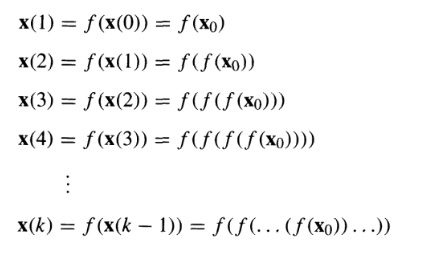
\includegraphics[width=90mm]{images/dynamical_systems_iteration.png}
    \caption{Iterating $f(x)$ to find the value of $x$ at time $k$.}
    \label{fig:dynamical_systems_iteration}
\end{figure}


% General form of discrete dynamical system:
% \begin{equation}
%     f(x(t)).
% \end{equation}

\subsection{Topics for further learning:}
Differential equations.

\subsection{Resources:}
Helpful indtroduction to dynamical systems: https://www.youtube.com/watch?v=A6R183ZIxC8
Invitation to dynamical systems by ER Scheinerman
Berkeley research on dynamical systems and machine learning: https://www.stat.berkeley.edu/~mmahoney/talks/dynamical_systems_and_ml_2.pdf

\end{document}